% Multiple Choice Question 12

\begin{center}
    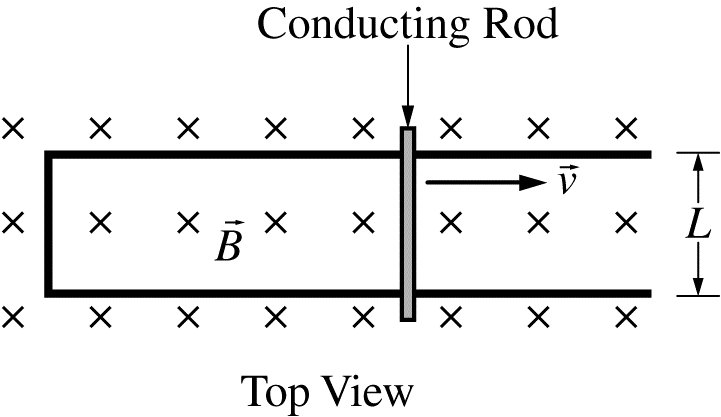
\includegraphics[scale=0.3]{images/img-007-014.png}
\end{center}

\begin{questions}
\setcounter{question}{11}

\question
A conducting rod of resistance $R$ is in electrical contact with a frictionless U-shaped rail of width $L$ and negligible resistance. The rod is pulled to the right at a constant velocity $\vec{v}$. A magnetic field $\vec{B}$ is directed into the page, as shown in the figure above. Under these conditions, the electric power dissipated in the rod is $P$. If the velocity of the rod is doubled, the power dissipated in the rod is

\begin{oneparchoices}
    \choice $P / 4$
    \choice $P / 2$
    \choice $P$
    \choice $2P$
    \choice $4P$
\end{oneparchoices}
\end{questions}
